\documentclass[11pt]{beamer}
\author{Philipp Arras, Florian Nowak}
\title{\LaTeX -Kurs}
\date{11. Oktober 2014}

\usetheme{Berkeley}
%\setbeamercovered{transparent}
\setbeamertemplate{navigation symbols}{}
%\logo{}
%\institute{}
%\subject{}

\usepackage[utf8]{inputenc}
\usepackage[ngerman]{babel}
\usepackage{amsmath,amsfonts,amssymb}
\usepackage{graphicx,booktabs}
\usepackage{wasysym}


\begin{document}

%\begin{frame}
%\titlepage
%\end{frame}

%\begin{frame}
%\tableofcontents
%\end{frame}

\section{Workflow}

\begin{frame}{Aufteilung}
\begin{itemize}
\item[$-$] Nachteil von {\TeX}: lange Dokumente werden unübersichtlich
\end{itemize}
\end{frame}

\begin{frame}{Aufteilung}
\begin{itemize}
\item[$-$] Nachteil von {\TeX}: lange Dokumente werden unübersichtlich
\item[$+$] Vorteil von {\TeX}: Teile des Dokuments können in externe Dateien ausgelagert werden
\end{itemize}
\end{frame}

\begin{frame}{Aufteilung}
\begin{itemize}
\item Um riesige Dateien zu vermeiden: Quellcode gemäß Inhalt aufteilen
\item Eine \emph{Hauptdatei} als leeres Gerüst
\item Eine \emph{header}-Datei (klare Trennung von Inhalt und {\TeX}nik; eventuell aufgeteilt in eine Datei für Formatierung, eine für Pakete und eine für Definitionen)
\item Inhalte in einem Unterordner nach strukturierter Anordnung
\item Abbildungen, sonstige Materialien in weiteren Unterordnern
\end{itemize}
\end{frame}

\begin{frame}{Aufteilung}
\begin{itemize}
\item Um riesige Dateien zu vermeiden: Quellcode gemäß Inhalt aufteilen
\item Eine \emph{Hauptdatei} als leeres Gerüst
\item Eine \emph{header}-Datei (klare Trennung von Inhalt und {\TeX}nik; eventuell aufgeteilt in eine Datei für Formatierung, eine für Pakete und eine für Definitionen)
\item Inhalte in einem Unterordner nach strukturierter Anordnung
\item Abbildungen, sonstige Materialien in weiteren Unterordnern
\item \emph{Alles}, was man im Rahmen der Arbeit braucht, sollte innerhalb eines Ordners (plus Unterordnern) liegen!
\item sync{\TeX} hilft, in die jeweils richtige Datei zu springen
\end{itemize}
\end{frame}

\begin{frame}{Beispiel Aufteilung}
\begin{figure}[h]
\centering
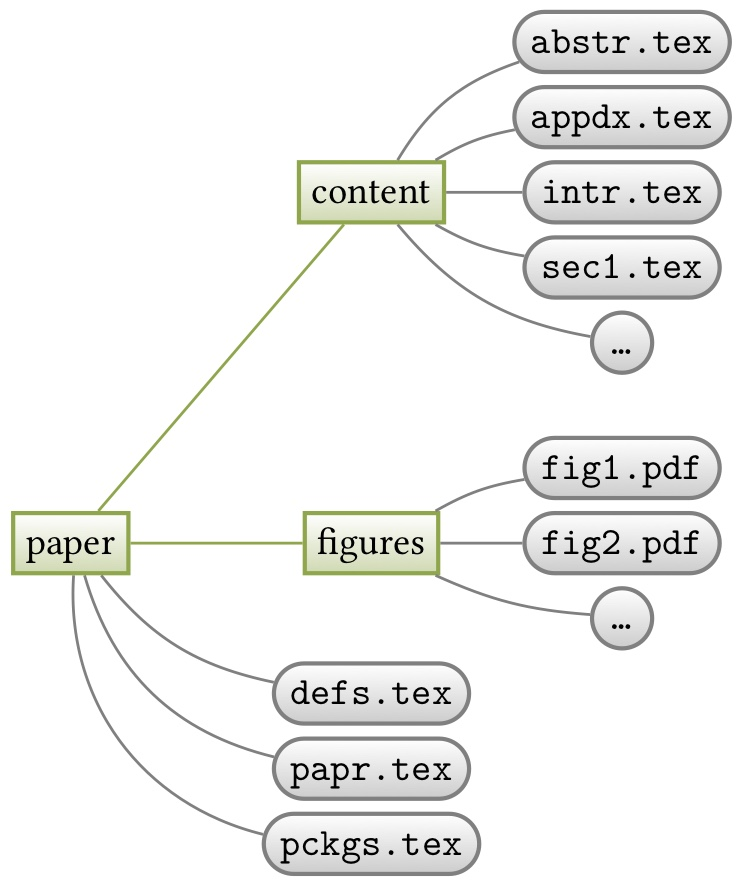
\includegraphics[scale=.235]{Ordnerstruktur}
\end{figure}
\end{frame}

\begin{frame}[fragile]{input und include}
\begin{itemize}
\item \verb~\input{...}~ und \verb~\include{...}~ führen externe Dateien am angegebenen Ort aus
\item {\TeX} {\glqq}springt{\grqq} aus dem aktuellen Dokument, liest woanders, und springt wieder zurück
\end{itemize}
\end{frame}

\begin{frame}[fragile]{input und include}
\begin{itemize}
\item \verb~\input{...}~ und \verb~\include{...}~ führen externe Dateien am angegebenen Ort aus
\item {\TeX} {\glqq}springt{\grqq} aus dem aktuellen Dokument, liest woanders, und springt wieder zurück
\item \verb~\input~ liest den Code einfach ein, als gehöre er zum Hauptdokument
\item \verb~\include~ erstellt eine eigene \texttt{.aux}-Datei\\
(sinnvoll, wenn \texttt{.aux} benötigt)
\end{itemize}
\end{frame}

\begin{frame}[fragile]{Beispiel Hauptdatei}
\begin{verbatim}
% papr.tex

\documentclass[ngerman]{scrartcl}
\input{pckgs}
\input{defs}
  
\begin{document}
  \include{abstr}
  \include{intr}
  
  \include{sec1}
  ...
  
  \include{appdx}
\end{document}
\end{verbatim}
\end{frame}

\begin{frame}{root Dokument}
\begin{itemize}
\item Nach Aufteilung muss immer das Hauptdokument kompiliert werden
\item[$-$] Nachteil: ständiges Wechseln zwischen Dokumenten nötig
\end{itemize}
\end{frame}

\begin{frame}{root Dokument}
\begin{itemize}
\item Nach Aufteilung muss immer das Hauptdokument kompiliert werden
\item[$-$] Nachteil: ständiges Wechseln zwischen Dokumenten nötig
\item[$+$] Vorteil durch sync{\TeX}: Springen zur gewünschten Stelle {\glqq}über{\grqq} PDF möglich
\end{itemize}
\end{frame}

\begin{frame}{Übung}
Dieses Mal keine {\smiley}
\end{frame}


\end{document}